\documentclass[12pt,a4paper]{article}
\usepackage{geometry}
\geometry{left=2.5cm,right=2.5cm,top=2.0cm,bottom=2.5cm}
\usepackage{CJKutf8}
\usepackage[english]{babel}
\usepackage{amsmath,amsthm}
\usepackage{amsfonts}
\usepackage[longend,ruled,linesnumbered]{algorithm2e}
\usepackage{fancyhdr}
\usepackage{array}
\usepackage{listings}
\usepackage{color}
\usepackage{graphicx}
\graphicspath{ {./images/} }

\begin{document}
\begin{CJK*}{UTF8}{gbsn}

\title{
  {《算法分析与设计》第 {$2$} 次作业
    \footnote{要求:1、分析题请用书面化语言给出详细分析过程。2、作业请统一使用hw0*-学号-姓名的命名格式,latex版本请附上源代码并打包提交。}
    }
}
\date{}

\author{
姓名:\underline{王骏}~~~~~~
学号:\underline{71119138}~~~~~~
成绩:\underline{~~~~~~~~~~~~~~~~~~}
}

\maketitle

\noindent
\section*{\bf \color{red}{算法分析题}}
\noindent
{\bf 题目1:}(1)用主方法解以下递推关系。
\begin{enumerate}
	\item[(a)]  $T(n)=4T(n/2)+n^2$
	\item[(b)]  $T(n)=3T(n/9)+5\sqrt{n}$
	\item[(c)]  $T(n)=4T(n/2)+n^2\sqrt{n}$
\end{enumerate}
(2)用迭代法获得以下递推关系的一个渐近上界。
\begin{enumerate}
	\item[(a)]  $T(n)=T(n/2)+2T(n/4)$
\end{enumerate}

\vspace{5pt}
\noindent
{\bf 答:}


(1)(a) 

$$ a = 4, b = 2, f(n) = n^2$$

$$ n^{\log_ba} = n^2 $$

for 
$$ f(n) = \Theta(n^2)$$

so
$$ T(n) = \Theta(n^2logn)$$

\vspace{5pt}

(1)(b)

$$ a = 3, b = 9, f(n) = 5\sqrt{n}$$

$$ n^{\log_ba} = \sqrt{n} $$

for 

$$ f(n) = \Theta(\sqrt{n})$$

so

$$ T(n) = \Theta(\sqrt{n}logn)$$

\vspace{5pt}

(1)(c)

$$ a = 4, b = 2, f(n) = n^2\sqrt{n}$$

$$ n^{\log_ba} = n^2 $$

for when $\varepsilon=\frac{1}{2}$

$$ f(n) = \Omega(n^{log_ba + \varepsilon})$$

$$af(\frac{n}{b}) = n^2\sqrt{\frac{n}{2}}$$

so when $ n \rightarrow \infty, c = \sqrt{\frac{1}{2}} $

$$ af(\frac{n}{b}) = n^2\sqrt{\frac{n}{2}} \leq cf(n) = n^2\sqrt{\frac{n}{2}}$$

so

$$T(n) = \Theta(f(n)) = \Theta(n^2\sqrt{n}) $$

\vspace{5pt}
(2)(a)

set 
$$n = 2^k$$

then
$$T(2^k) = T(2^{k-1}) + 2T(2^{k-2})$$

mark 

$$T(2^k) = M(k)$$

then

$$M(k) = M(k-1) + 2M(k-2)$$

so the characteristic equation

$$x^2 = x + 2$$

solve it then

$$
\left\{\begin{array}{lcl}
		x_1 = 2\\
		x_2 = -1
\end{array}\right
$$

so 

$$
M(k) = \alpha2^k + \beta(-1)^k
$$

$$M(k) = \Mathcal{O}(2^k)$$

then

$$T(2^k) = \Mathcal{O}(2^k)$$

so

$$T(n) = \Mathcal{O}(n)$$

\vspace{10pt}
\noindent
{\bf 题目2:}解递推关系 $T(n)=2T(\sqrt{n})+lgn$。
\vspace{5pt}
\noindent
{\bf 答:}

The recursive tree:\\

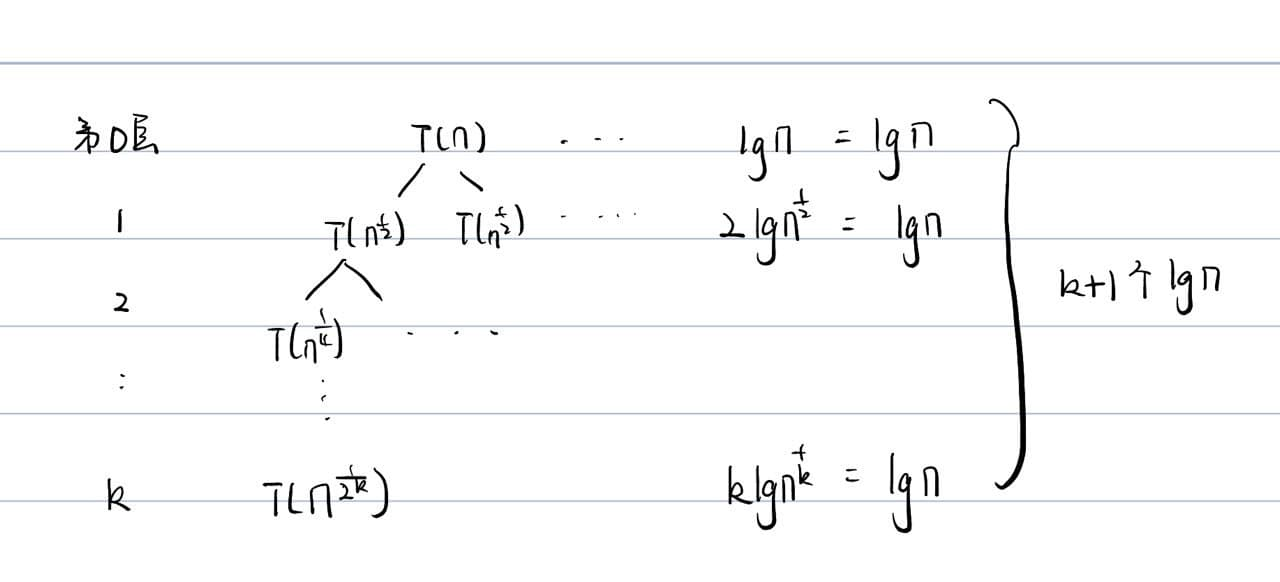
\includegraphics[width=15cm]{pic_hw2.jpg}

when n = 1

$$T(1) = 2T(1)$$

so 

$$T(1) = 0$$

and 

$$\lim_{n \to +\infty} n^{\frac{1}{n}} = 1$$

so when $k = \log_2n$

$$T(n^{\frac{1}{2^k}}) = T(1) = 0$$

so 

$$T(n) = (k+1)lgn = (\log_2n+1)lgn$$

\vspace{10pt}
\noindent
{\bf 题目3:}用分治法设计一个算法找出数组 $A[1..n]$ 中的最大的数,并分析所需的比较次数。(需先设计出算法,再分析比较次数)

\vspace{5pt}
\noindent
{\bf 答:}

Algorithm:\\

不停地将数组二分,然后比较二分后两个子数组的最大值\\

Analysis:\\

\left\{\begin{array}{lcl}
		T(n) = 2T(\frac{n}{2}) + 1\\
		T(2) = 1
	\end{array}\right\\

Recurisve Tree:

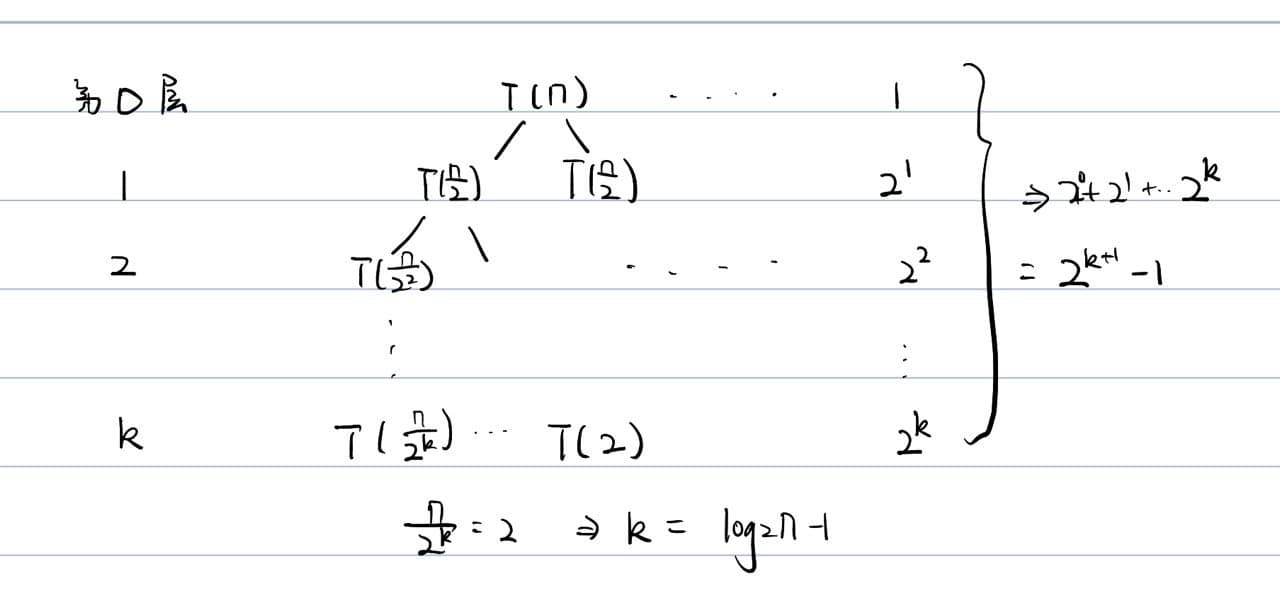
\includegraphics[width=15cm]{pic_hw3.jpg}

so

$$
T(n) = 1 + 2^1 + ... 2^k = 2^{k+1} -1\\
= 2^{log_2n - 1 + 1} -1 = n -1 = \Theta(n)
$$

\end{CJK*}
\end{document} 
